\documentclass{report} 
\usepackage{graphicx}

\begin{document}

\begin{titlepage}
\begin{center}
{ \vspace*{3cm} }
%\vspace{3cm}
{\Huge GAMETES User's Guide}\\[0.5cm]
{\LARGE Version 2.1 Beta}\\[1.5cm]
{\large Ryan J Urbanowicz$^1$ and Geoffrey Kiralis$^2$ and Jonathan M Fisher$^3$ and Jason H Moore$^4$}\\[0.5cm]
{\large \today}\\
\vfill
% Bottom of the page
\end{center}
\begin{flushleft}
$^1$ryan.j.urbanowicz@dartmouth.edu - Algorithm and Software Development\\
$^2$geoffrey.kiralis@dartmouth.edu - Algorithm Development\\
$^3$jonathan.fisher@dartmouth.edu - Software Development\\
$^4$jason.h.moore@dartmouth.edu - Principle Investigator
\end{flushleft}
\end{titlepage}

\newpage
\addtocontents{toc}{\protect\enlargethispage{35mm}}
\tableofcontents

\newpage

%SELF NOTES*************************************
%what happens when you make model with one locus - i ran one and heritability seemed wrong... is it working?? her calc??
%default att number to 2
%quantile pop size - if it's 1 or not many - have a minimum search size of like 1000, or 10000
%non-predictive attributes box should only  be up to balanced case/control button.
%read from file. format?? does it work??
%View snp file doesn't seem to work
%Format of real data files

\chapter{Introduction}   
\section{What is GAMETES?} 
Genetic Architecture Model Emulator for Testing and Evaluating Software (GAMETES) is a fast direct algorithm for the generation of complex single nucleotide polymorphism (SNP) models for simulation studies.  In particular, GAMETES is designed to generate epistatic models which we refer to as pure and strict.  Purely and strictly epistatic models constitute the worst-case in terms of detecting disease associations, since such associations may only be observed if all \emph{n}-loci are included in the disease model.  This makes them an attractive gold standard for simulation studies considering complex multi-locus effects.  The user friendly GAMETES software affords users the ability to rapidly and precisely generate epistatic multi-locus models, as well as the option to generate simulated datasets based on these models. In version 2, we have added the ability to generate heterogeneous datasets by applying multiple independent models to different subsets of the simulated data.  Additionally we have added a custom model generation feature, so that users may directly specify and examine the properties of any 2 or 3 locus SNP model. Simple main effect models (i.e Mendelian) may also be generated with this feature.

\section{Algorithm Overview} 
The core GAMETES algorithm provides a direct approach for the simulation of biallelic \emph{n}-locus epistatic models which may be used in conjunction with any sample generation strategy.  Each \emph{n}-locus model is generated deterministically, based on a set of random parameters, a randomly selected direction, and specified values of heritability, minor allele frequencies, and population disease prevalence.  For valid combinations of these model constraints, GAMETES attempts to generate a population of model architectures.  We use the term \emph{architecture} to reference the unique composition of a model (i.e. the penetrance values and arrangement of those values across genotypes).  This algorithm was designed to maximize the randomness of model generation, given a desired set of genetic constraints.

\section{Further Reading} 
\begin{itemize}
\item  For a complete description of the GAMETES algorithm and an example simulation study, see \cite{urbanowicz2012gametes}.
\item  For a complete description of the difficulty metric adopted by GAMETES for model selection, see \cite{urbanowicz2012predicting}.
\item  For early applications of the GAMETES model/data simulation strategy to a simulation study, see \cite{urbanowicz2010application,urbanowicz2011application}.
\item For a classification and characterization of 2-locus models, an examination of the relationship between model `shape' and model detection difficulty, and an exploration of how model population size and population prevalence impact model diversity in GAMETES, see \cite{urbanowicz2013classification}
\end{itemize}

\section{Obtaining the Software}
GAMETES 2.1 is available as an open-source (GPL) software package.  It is a cross-platform program written entirely in Java.  It is freely available for download from http://sourceforge.net.  You may also contact Dr. Jason Moore for a copy of the software or source code if you experience difficulties downloading it from the web site.

\section{Minimum System Requirements} 
\begin{itemize}
\item  Java Runtime Environment, version 5.0 or higher (http://www.java.com/).
\item  1 GHz processor
\item  256 MB Ram
\item  800x600 screen resolution
\end{itemize}

\section{GAMETES Versions} 
\textbf{Version 1.0:} Made available on 1/16/2012. Original version of algorithm/software.\\ \\
\textbf{Version 2.0:} Made available on 2/20/2014. Expanded version of GAMETES.
\begin{itemize}
\item  Added ability to combine genetic models and generate heterogeneous datasets.
\item  Added window to GUI to allow user to specify custom 2 or 3 locus models, or to edit existing 2 or 3 locus models.
\end{itemize} 
\textbf{Version 2.1:} Made available on 3/29/2014. Fixed dataset generation limitation.
\begin{itemize}
\item  In GAMETES 2.0, simulated datasets were being stored in memory during generation, limiting the algorithm's ability to generate datasets with greater than approximately 10,000 attributes.  This version avoids storing the entire dataset in memory, and thus has a much smaller memory footprint when generating large datasets.
\end{itemize}

\section{Starting the Program} 
After downloading the file, there will be a file called \texttt{GAMETES$\_$2.1.jar}.  Under most operating systems, simply double-clicking this file will be sufficient to start the program.  However, there are reasons a user may wish to start the program from the command line.  To do so, open a command shell and navigate to the directory containing \texttt{GAMETES$\_$2.1.jar}.  Issue the command:
\begin{center}
\texttt{java -jar GAMETES$\_$2.1.jar}
\end{center}
To open the command line help for GAMETES, give the command:
\begin{center}
\texttt{java -jar GAMETES$\_$2.1.jar -h}
\end{center}
Running GAMETES from the command line requires arguments which are discussed in section \ref{cmdop}.  The option to run GAMETES from the command line with no graphical user interface (GUI) facilitates the generation of an extensive model/dataset archive.

\chapter{Using GAMETES}   
\section{GAMETES GUI Overview} 
When you open the GAMETES GUI, you will see the window given in Figure \ref{gui}.  The GUI is divided into a top half, dedicated to model generation, and a bottom half dedicated to dataset generation.  The GAMETES GUI may be used to (1) generate new models, (2) generate datasets from an existing model, or (3) both tasks.  As seen in Figure \ref{gui}, when you first start GAMETES, the \texttt{Model Construction} box is empty (i.e. there are no model files opened).  Whether your task is model or dataset generation, begin by opening a model in the \texttt{Model Construction} box.  This is accomplished by clicking one of three buttons at the top of the GUI: (1) \texttt{Generate Model} (2) \texttt{Create Model}, or (3) \texttt{Load Model}.  The \texttt{Generate Model} button will open a secondary window for applying the GAMETES algorithm to generate a model as discussed in section \ref{modgen}.  Once a new model has been saved it will automatically open in the \texttt{Model Construction} box (see Figure \ref{modop}).  The \texttt{Create Model} button will open a secondary window for specifying or editing a custom 2 or 3 locus model.  Similarly, a model saved from this window will automatically open in the \texttt{Model Construction} box.  The \texttt{Load Model} button brings up a file browser, which allows you to navigate to and select a previously saved model file.  Note that model files saved in GAMETES have file names with '$\_$Models' added to distinguish them as a properly formatted model file.

\begin{figure}[t]
\centering
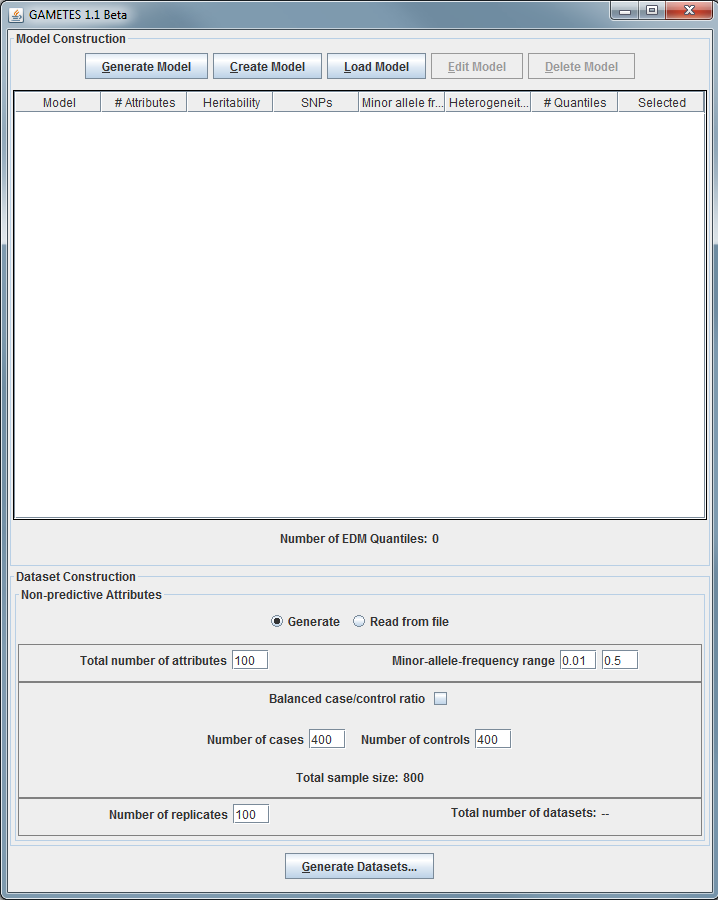
\includegraphics[width=0.8\textwidth]{Figure1_UG.png}% %16.6  
\caption{GAMETES GUI screenshot.}
\label{gui}
\end{figure}

\begin{figure}[t]
\centering
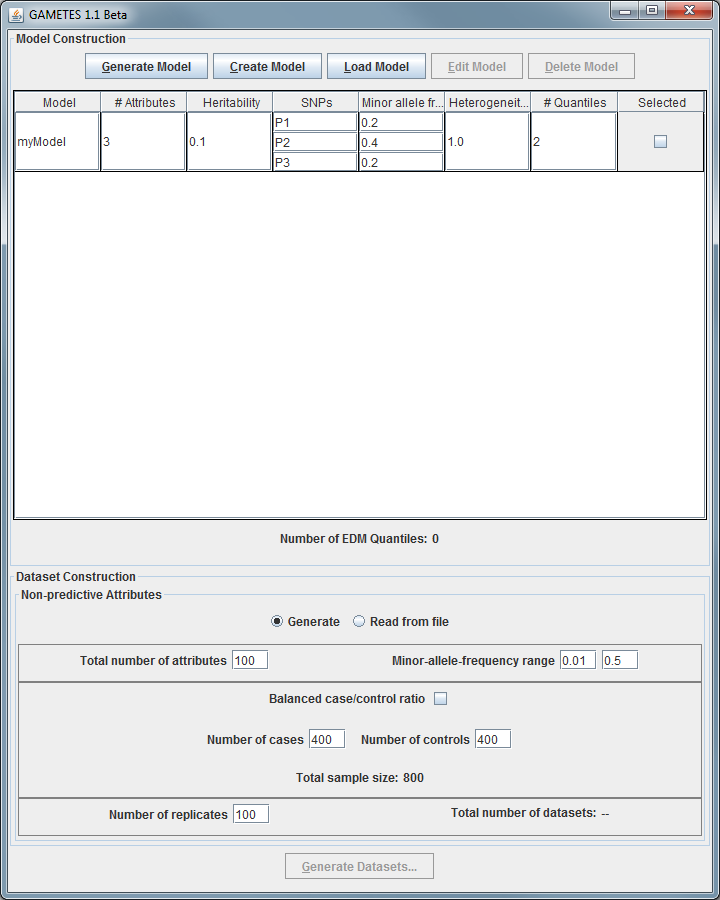
\includegraphics[width=0.8\textwidth]{Figure2_UG.png}% %16.6  
\caption{Model opened in the model construction box.}
\label{modop}
\end{figure}

The \texttt{Edit Model}, and \texttt{Delete Model} buttons only become available once a model has been loaded into the \texttt{Model Construction} box, and the user has selected the check box for the model they wish to edit or delete.  The \texttt{Edit Model} button opens the same secondary window as \texttt{Create Model}, but instead of a blank model, the selected model is opened for editing.  \texttt{Edit Model} is only available for models with 2 or 3 loci (loci are also referred to as attributes), and that have a respective model file with a \texttt{Quantile Count} of 1.  Of note, GAMETES model files can contain multiple models (i.e. penetrance functions) based on the \texttt{Quantile Count} specified by the user. \texttt{Quantile Count} is discussed further in section \ref{oparm}.  Lastly, the \texttt{Delete Model} button clears a selected model file from the \texttt{Model Construction} box, but does not delete the respective model .txt file that was also generated.  

Towards the top of the \texttt{Model Construction} box, notice the column headers which describe the properties of the opened model file(s).  These include (1) \texttt{Model}, an arbitrary model identifier, (2) \texttt{$\#$ Attributes}, (3) \texttt{Heritability}, (4) \texttt{SNPs}, the number of loci included in the model, (5) \texttt{Minor allele frequencies}, for each attribute, and (6) \texttt{Heterogeneity proportion}, used in generating heterogeneous data, (7) \texttt{ $\#$ Quantiles}, the number of models in the respective model file,  and (8) \texttt{Selected}, a checkbox for selecting specific models loaded in the window.  Of note, \texttt{Heterogeneity proportion} and \texttt{Selected} are the only columns in the \texttt{Model Construction} box with an editable field.

The next three sections details the major components of the GUI as follows: (1) the generation of models using the core GAMETES algorithm (section \ref{modgen}), (2) the creation and editing of custom models (section \ref{custmod}), and (3) dataset generation, including the generation of heterogeneous datasets (section \ref{datgen}).

\section{Model Generation}\label{modgen}
When the \texttt{Generate Model} button is selected, the window like the one shown in Figure \ref{modgenP} will appear.  This window allows the user to specify constraints of the genetic model(s) they wish to generate.  By default, this window will open with simple model constraints specified that will yield valid 2-locus models (heritability of 0.2, and minor allele frequencies of 0.2).  The user has the option to edit the following items; (1) number of attributes, (2) heritability, (3) minor allele frequencies, (4) population prevalence, (5) the name of the SNP, (6) the model difficulty metric used to identify quantiles, (7) the quantile count, and (8) quantile population size.  These are all discussed below.  To modify one of the default model constraints,  click on the respective box and type in a new value.  Double clicking one of these boxes will highlight the contents of the box and allow the user to directly replace the existing value.  Figure \ref{modgenP} gives a model generation window that has been edited to specify a model with 3 attributes, a heritability of 0.1, and minor allele frequencies of 0.2, 0.4, and 0.2 respectively.

\begin{figure}[t]
\centering
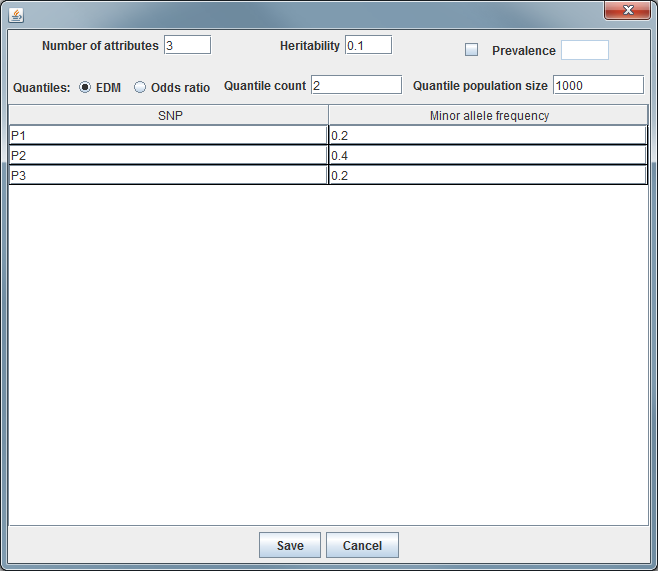
\includegraphics[width=0.8\textwidth]{Figure3_UG.png}% %16.6  
\caption{Model generation window.}
\label{modgenP}
\end{figure}

\subsection{Number of attributes}
\texttt{Number of attributes} refers to the number of SNPs which are to be included in the model.  After changing the number of attributes, click on any other white space in the window for the change to take effect. You will see additional rows appear in the model window as you increase this value.  

\subsection{Heritability}
\texttt{Heritability}, or the (broad-sense) heritability of a genetic model is the proportion of observable differences between individuals that is due to genetic differences.  Keep in mind that as you select higher values of heritability it becomes less likely that GAMETES will be able to randomly generate such models since GAMETES has the ability to scale a model down to the desired heritability, but not up.  See \cite{urbanowicz2012gametes} for more details.  

\subsection{Population Prevalence}
Population prevalence (K) is the proportion of individuals in a population that have the disease of interest.  Note that GAMETES gives the user the option to leave K unspecified, in which case the K of the models that are generated will vary.  To specify K, select the check-box to the left of \texttt{Prevalence} and then specify a value of K between 0 and 1. Previous analysis of simulated models suggests that K has a negligible impact on model difficulty.  Allowing K to vary also facilitates GAMETES's ability to find models with a precise set of model constraints (particularly important for models with a higher heritability or larger number of attributes) \cite{urbanowicz2013classification}.  Additionally, dataset samples are generated according to user defined quantities of cases and controls, and thus the K of a model will not impact the case/control balance in the dataset.  For these three reasons, we suggest leaving K unspecified in most situations.

\subsection{Minor Allele Frequency}
The minor allele frequency (MAF) is the frequency at which the less common allele occurs in a given population.  Once the user has specified number of attributes, adjust the MAF for every SNP in the model to the desired value between 0 and 0.5.

\subsection{Other Parameters}\label{oparm}
While GAMETES gives a default name for each SNP in the model (e.g. P1, which stands for Predictive SNP 1) you may modify each name, again by clicking on the respective cell and typing in a new name. The remaining parameters deal with the population of models to be generated, and how a model or models will be selected and saved.  First, \texttt{Quantiles} is an option with two radio buttons indicating 'EDM' or 'Odds Ratio'.  This simply selects the difficulty metric that will be used to rank models in the population to be generated.  See Section \ref{moddiff} for more on these metrics. Second, \texttt{Quantile Count} refers to the number of random model architectures you wish to save to the model output file (which may subsequently used to generate simulated datasets).  Third, \texttt{Quantile Population Size} refers to the number of random model architectures you want GAMETES to try and generate for the given model constraints.  If you wish to generate a single random model (with the specified model constraints) set \texttt{Quantile Count} and \texttt{Quantile Population Size} both to 1.  Each model that is successfully generated will satisfy the model constraints given, but will possess a unique random architecture.   If you want GAMETES to save all model architectures it generates, set \texttt{Quantile Count} equal to \texttt{Quantile Population Size}.  Setting \texttt{Quantile Count} to a lower value than \texttt{Quantile Population Size} will direct GAMETES to choose a subset of the random models to be saved.    This selection process is based on a model difficulty metric discussed in section \ref{moddiff}.  In short, N random models (where N = \texttt{Quantile Population Size}) are ordered by their difficulty and X models are reported/saved (where X = \texttt{Quantile Count}).  \texttt{Quantile Count} may not be larger than \texttt{Quantile Population Size}.  If \texttt{Quantile Count} = 1, the model with the median "difficulty" is reported.  If \texttt{Quantile Count} = 2, the models with the maximum and minimum "difficulties" are reported.  If \texttt{Quantile Count} = 3, the maximum, minimum, and median models are reported.  Larger values of \texttt{Quantile Count} select models at evenly spaced intervals.

\subsection{Saving Models}\label{saving}
Once all parameters have been specified, click \texttt{Save}.  This will bring up a file browser, which allows you to select the name and destination for your model file.  Model files are saved as \texttt{FileName\textunderscore Models.txt}. In addition to the models file, a secondary .txt file will be saved that gives the model difficulty scores for all N models generated for the given combination of model constraints.  These files are saved as \texttt{FileName\textunderscore EDM\textunderscore Scores.txt} or \texttt{FileName\textunderscore OddsRatio\textunderscore Scores.txt} depending on the difficulty metric you select.  When searching for models, a progress bar will appear which indicates the proportion of search attempts GAMETES has made.  This does not necessarily reflect the number of models it has successfully found during the course of running.

\section{Custom Models}\label{custmod}
\begin{figure}[t]
\centering
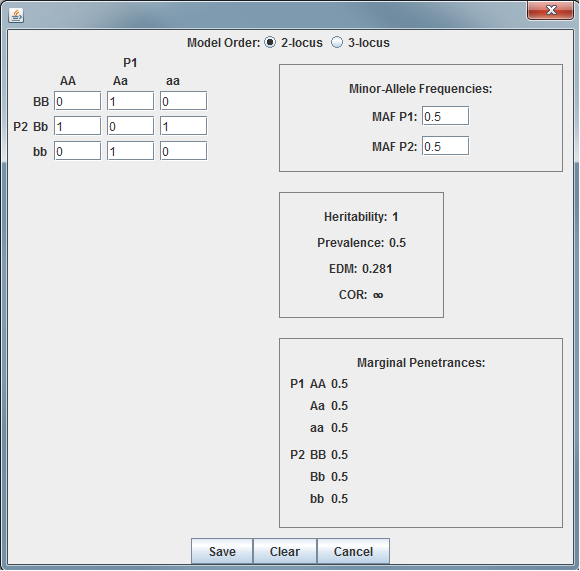
\includegraphics[width=0.8\textwidth]{Figure4_UG.png}% %16.6  
\caption{Custom model window (2-locus model).}
\label{cust2}
\end{figure}
When either the \texttt{Create Model} or \texttt{Edit Model} button is selected, a window like the one shown in Figure \ref{cust2} will appear.  This window allows the user to specify or edit a custom model.  This feature is only available for generating or editing model files with a \texttt{Quantile Count} of 1.  If \texttt{Create Model} is selected, the initial model will be blank (i.e. all penetrance values will be zero), while if \texttt{Edit Model} is selected, the the selected model will be opened for editing (however for readability, only a few decimal places from the original model file will be preserved).  This window allows the user to edit three aspects of a given model: (1) the model order, i.e. the number of attributes in the model (limited to 2 or 3 attributes), (2) the penetrance values of the penetrance function (penetrance is the probability of disease if a individual has a particular genotype combination), and (3) the minor allele frequencies of each attribute.  To change model order, click on the appropriate radio button.  Note that when the 3-locus option is selected the dimensionality of the penetrance function is updated accordingly (see Figure \ref{cust3}).  Also, note that genotypes for each attribute are either labeled ([AA, Aa, aa], [BB, Bb, bb], or [CC, Cc, cc]).  Attributes themselves are labeled by default as P1,P2,or P3 for each 'predictive' SNP in the model.  To modify penetrance or minor allele frequency values, click on the respective box and type in a new value.  Double clicking one of these boxes will highlight the contents of the box and allow the user to directly replace the existing value.  The user may also hit the Tab key to shift from one box to the next.  

\begin{figure}[t]
\centering
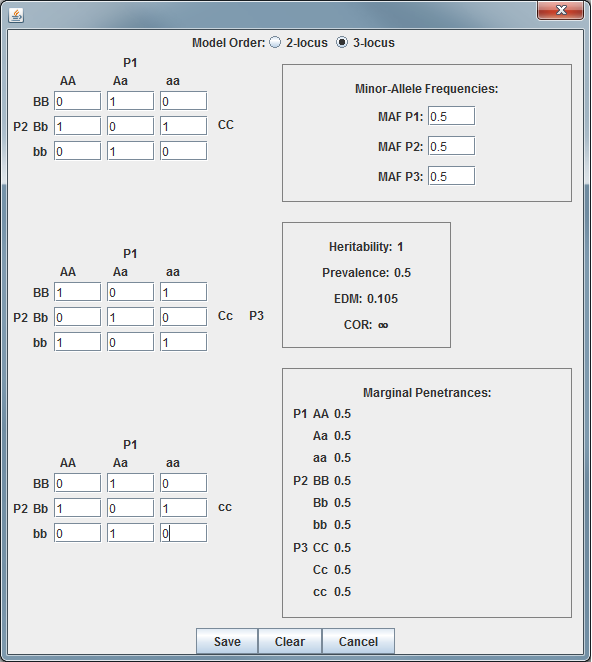
\includegraphics[width=0.8\textwidth]{Figure5_UG.png}% %16.6  
\caption{Custom model window (3-locus model).}
\label{cust3}
\end{figure}

The custom model window also includes feedback on the properties of the currently specified model.  This includes heritability, population prevalence, two difficulty metrics (EDM and COR discussed further in section \ref{moddiff}), and the marginal penetrances of the model.  Marginal penetrances give the probability of disease for each geneotype when when considering only a single attribute at a time.

Saving custom models is achieved as described in section \ref{saving}, however it is important to keep in mind that when creating or editing custom models, all saved model files will include only that single model, giving all such model files a \texttt{Quantile Count} of 1.

Also, please note that based on how the COR difficulty metric is calculated, it is possible for the calculation of the ratio to become mathematically impossible, at which point a value of infinity is assigned within the \texttt{Create Model} window.  This occurs when either the number of false positives, or the number of false negatives in the model is zero.  This is true for all fully penetrant models (models where all penetrance values are either 0 or 1).  To clarify further, a fully penetrant genotype (i.e. cell in the model) with a value of 1 yields no false negatives, while a genotype with a penetrance of 0 yields no false positives.  If a cell has a penetrance larger the the population prevalence, than that cell contributes either false negatives or true positives.  If a cell has a penetrance smaler than the population prevalence, then the cell contributes either false positives or true negatives.  For more information on the COR metric, please see \cite{urbanowicz2012predicting}.

\section{Dataset Generation}\label{datgen}
We begin by describing how to generate datasets from a single model.  Later in section \ref{hetdata} we will explain how to combine multiple models in order to generate heterogeneous datsets.

Once a single model has been opened and selected in the \texttt{Model Construction} box, you may generate simulated datasets derived from that model.  No matter how many models are loaded in the \texttt{Model Construction} box, only the one that is 'selected' will be used to generate datesets.  Notice that once a model is 'selected' the \texttt{Number of Quantiles} for the loaded model is displayed at the bottom of the \texttt{Model Construction} box.  Datasets simulated using GAMETES have two types of attributes/SNPs, (1) predictive attributes, and (2) non-predictive attributes.  Predictive attributes are those specified in the genetic model.  Non-predictive attributes are all other attributes which have no specified association with affection status (i.e. case or control).  The first step is to decide how to include non-predictive attributes.  Select the radio button, \texttt{Generate} to randomly generate genotypes for all non-predictive attributes.  Select the radio button \texttt{Read from file} to use an existing real or simulated SNP dataset as the non-predictive attributes.  

\subsection{Randomly Generate Non-Predictive Attributes}
If \texttt{Generate} is selected the GAMETES window will appear as in Figure \ref{modop}.  If \texttt{Generate} is selected then you must also specify the \texttt{Total number of} \texttt{attributes}.  This is the total number of SNPs which will appear in each simulated dataset.  This number includes all predictive attributes included in the model.  E.g.  If you have a 3-locus model, and you specify 100 total attributes, 97 will be non-predictive.  Additionally, select the \texttt{Minor-allele-frequency range}.  The MAF of each non-predictive attribute is randomly selected from within this range with uniform probability.  Next if an equal number of cases and controls is desired, check the box for \texttt{Balanced case/control ratio}.  This will restrict the number of controls, such that it is the same as the number of cases.  Adjust \texttt{Number of cases} and \texttt{Number of controls} by double-clicking the respective box and entering the desired value.  If \texttt{Balanced case/control ratio} is checked, a change in \texttt{Number of cases} will appear in \texttt{Number of controls} when you click in the white space of a separate box.  Once you have done so, the \texttt{Total sample size} will update it self to reflect the correct total. Finally, specify the \texttt{Number of replicates}.  This is the number of randomly seeded simulated datasets which will be generated for each of the genetic models.  \texttt{Total number of datasets} indicates the number of datsets which will be generated when the user clicks \texttt{Generate Datasets...} at the bottom of the window.  If the user has selected 3 model quantiles, and 100 replicates, a total of 300 datasets will be generated (100 for each of three models with different architectures, but the same set of model constraints).  Next, click \texttt{Generate Datasets...}.  This will bring up a file browser, which allows you to select the name and destination for folders which will contain your saved datasets (one folder for each quantile).  Finally, click \texttt{Save} and a progress bar will appear as datasets are generated and saved.  Notice that by default, the datasets are saved such that the first columns include non-predictive attributes, followed by predictive attributes, and lastly the class status.  Non-predictive attributes are labeled in the dataset with the prefix 'N' (e.g. N38).  Predictive attribute labels begin with a simple model identifier (useful when modeling heterogeneity), with the prefix 'M' for model, and then the prefix 'P' for predictive attribute (e.g. M0P4).

\subsection{Load Non-Predictive Attributes}\label{loaddata}
\begin{figure}[t]
\centering
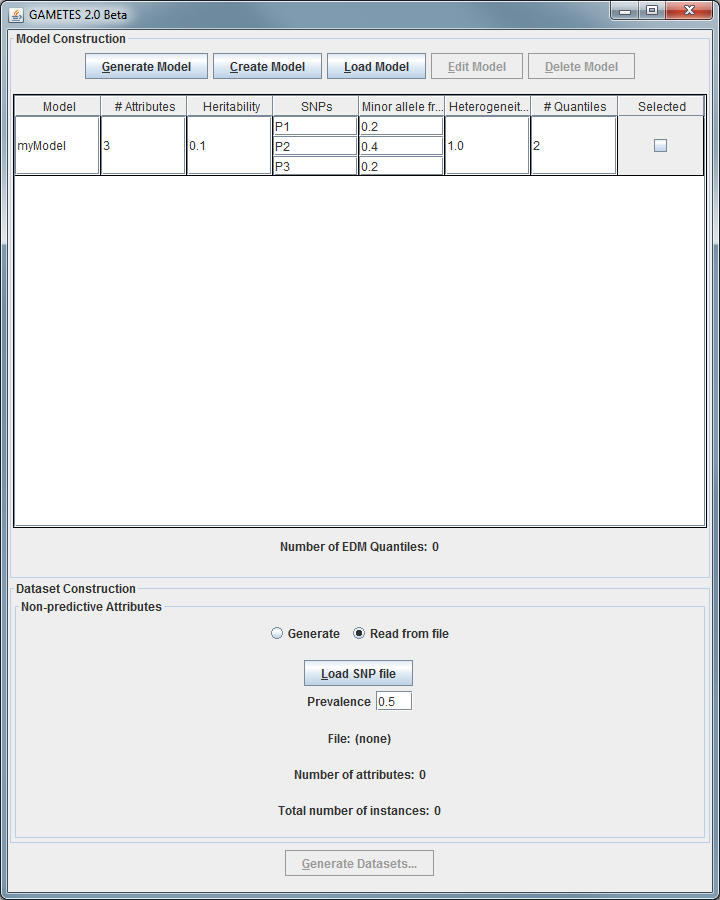
\includegraphics[width=0.8\textwidth]{Figure6_UG.png}% %16.6  
\caption{Read from file options}
\label{readfile}
\end{figure}
If you select \texttt{Read from file}, the options in the lower half of the GAMETES window change (see Figure \ref{readfile}).  Selecting this option allows a user to load an existing file (such as a real SNP dataset) to be used as the non-predictive attributes.  Click \texttt{Load SNP file} to bring up a file browser, which allows you to navigate to and select an existing dataset. The current implementation of GAMETES requires the following format for loaded datasets:
\begin{itemize}
\item  Files should be tab-delimited text files.
\item  The first row of the file should contain header labels for all attributes/SNPs.
\item  Rows should denote subjects, and columns should denote attributes/SNPs.
\item  The three biallelic SNP genotypes should be encoded as 0,1,or 2.  There should be no other attribute values or missing data.
\item  The file should include attribute data only (no class label or status for any subject).
\end{itemize}

Once loaded, the \texttt{Number of attributes} and \texttt{Total number of instances} will be automatically determined, based on the dataset that has been loaded.  \texttt{Number of attributes} will equal the number of attributes in the loaded dataset only.  The number of attributes in the datasets that will be generated is \texttt{Number of attributes} plus the number of attributes in the loaded genetic model.  \texttt{Total number of instances} will be equal to the number of instances in the loaded dataset.  A small update in GAMETES 2.0, we have added the ability to adjust the case/control ratio when generating datasets in this manner.  To adjust the ratio of cases to controls in the dataset to be generated, adjust the \texttt{Prevalence} value between 0 and 1.  If the user sets \texttt{Prevalence} to 0.5, GAMETES will generate a balanced dataset (i.e. 50\% cases and 50\% controls) assuming the loaded dataset contained an even number of samples (if not GAMETES will generate a dataset as close to balanced as possible). A lower value will yield more controls, and a higher value will yield more cases.  Lastly, click \texttt{Generate Datasets...} to generate datasets as described above.  Notice that a model from the \texttt{Model Construction} box must be selected in order to generated datasets.

\subsection{Heterogeneous Datasets}\label{hetdata}
The first step to generate heterogeneous data is to load and select two or more models into the \texttt{Model Construction} box.  A new model may be added to this window as previously described by either generating, creating, or loading a model.  Note that while any number of models may be loaded into the \texttt{Model Construction} box, only models that are selected using the check boxes will be used to generate datasets.  Additionally, all selected model files must have the same number of quantiles (i.e. the same \texttt{Quantile Count}).  For example, if two models files are selected (each with two quantiles), heterogeneous datasets will be generated for both the high and low difficulty quantiles (where the high difficulty models are paired to make heterogeneous datasets, and the low difficulty models are similarly paired to make separate heterogeneous datasets.  Next, within this same window, adjust the values for the \texttt{Heterogeneity proportion} as desired.  This value indicates the relative proportion of the dataset which will be simulated based on the given model.  Any values entered into this field for respective models will be normalized with respect to each other.  For example if this value is set the same for each model, then GAMETES will attempt to generate a dataset with an equal number of samples having been generated from each model.  As another example, if the user has selected two models, and wants $75\%$ of the data from one model and $25\%$ from the other, they could simply specify a \texttt{Heterogeneity proportion} of 75 for the first and 25 for the second.  This is illustrated in Figure \ref{hetfile}.  When only a single model is selected in the \texttt{Model Construction} box, the \texttt{Heterogeneity proportion} has no impact on the datasets that are simulated.  This value is arbitrarily set as to 1.0 initially for each model in the window.  In order to generate and save the simulated datasets, carry on as previously described in the previous subsections.  Note that within saved heterogeneous datasets, predictive attribute names are modified with an arbitrary identifier that indicates which model the respective attributes came from.  For example instead of attributes from the first model being named P0 and P1, they will be named M0P0, and M0P1 while attributes from a second model would have the prefix 'M1'.  

\begin{figure}[t]
\centering
\includegraphics[width=0.8\textwidth]{Figure7_UG.png}% %16.6  
\caption{Generating heterogeneous datasets}
\label{hetfile}
\end{figure}

\section{EDM and COR} \label{moddiff}
A more recent feature to have been added to GAMETES is the ability to select a subset of representative models from a population of models with random architectures.   In developing and testing GAMETES, we observed that despite keeping all previously mentioned model constraints constant, an algorithm's detection proportion could vary greatly.  Detection proportion refers to the proportion of datasets within which the correct underlying model was identified.  One would observe higher proportions for detecting an "easier" model, than a more "difficult" model.  While some variation can be explained by the probabilistic translation of models into randomly seeded datasets, the rest can logically be attributed to subtle differences in model architecture.  GAMETES has two difficulty metrics implemented as options for model selection.  These include a customized odds ratio (COR), informally utilized in \cite{motsinger2008comparison} and \cite{edwards2009exploring}, as well as our Ease of Detection Measure (EDM), formally introduced and evaluated in \cite{urbanowicz2012predicting}.  Both metrics are calculated directly from the genetic model, and were found to demonstrate a strong, significant correlation with a given model's detectability.  Both metrics offer a viable method for model selection with no significant difference between them.  Also, for both metrics, a larger respective value indicates that the model should be easier to detect than a model with a lower value. 

\section{Model Output Files} 
Text files in which models are saved provide the following information for each model selected as a quantile by GAMETES: attribute names, MAFs, K, heritability, and both the EDM and COR score for the model.  Additionally the penetrance values for every genotype combination in the model are given as a penetrance function.  These penetrance functions can become difficult for a user to easily interpret as the number of loci (\emph{n}) is greater than 3.  If \emph{n} is 2, the genotypes of the first SNP are the rows of the penetrance function, while the genotypes of the second SNP are the columns.  If \emph{n} is 3, these positions shift.  The genotypes of first SNP are represented by the three 2-locus penetrance functions, the genotypes of the second SNP are the rows, and the genotypes of the third SNP are the columns.  If \emph{n} is 4, the genotypes of first SNP are now represented by the three, 3-locus penetrance functions.  This pattern continues as \emph{n} continues to increase, where the last of \emph{n} SNPs is always represented by the columns.  See Table 2.1 below for an example of a 2-locus penetrance function, where the function includes 9, or $3^n$, penetrance values.  Notice here how the rows represent genotypes of SNP 1, while columns represent genotypes of SNP 2.

\begin{table}[!h] \centering\caption{A 2-locus purely epistatic penetrance function.}\label{Pen2}
\begin{tabular}{p{1cm}c ||c | c | c || c }
&&\multicolumn{3}{c||}{SNP 2}&Marginal\\
&Genotype&BB(.25)&Bb (.5)&bb(.25)&Penetrance\\ \hline \hline
&AA(.36) & .266 & .764 & .664 & .614 \\ \cline{2-6}
SNP 1 &Aa (.48) & .928 & .398 & .733 & .614 \\ \cline{2-6}
&aa(.16) & .456 & .927 & .147 & .614 \\ \hline \hline
&Marginal & .614 & .614 &.614 & K = .614 \\
&Penetrance&&&&
\end{tabular}
\end{table}

\section{Limits of GAMETES} 
In \cite{urbanowicz2012gametes} we discuss specific limits of the GAMETES software.  In particular users should be aware that GAMETES's ability to generate genetic models is limited by what constraint combinations are mathematically possible, as well as which ones have a reasonable probability of being generated by chance.  We illustrate the limits of 2-locus model constraint combinations in Figure \ref{maxherfig} published in \cite{urbanowicz2012gametes}.  Presently if you wish to know if GAMETES can generate models with a particular set of model constraints, the best strategy is trial and error.  By default, the GAMETES GUI is alotted a \texttt{Number of Attempts} of 100,000 to find the desired number of models for \texttt{Quantile Population Size} requests up to 1000.  If the user requests population sizes larger than 1000, the maximum \texttt{Number of Attempts} becomes 100X the requested \texttt{Quantile Population Size}.  Alternatively, \texttt{Number of Attempts} may be precisely specified when running GAMETES from the command-line.  If GAMETES fails to find the number of models specified in \texttt{Quantile Population Size}, but that number is larger than {Quantile Count} (the number of models the user wanted specified in the model file), a warning message will appear notifying the user of the number of models it was able to find.  In this case a model file will still be generated, but GAMETES will select the number of models specified in {Quantile Count}, out of the population of models it was able to find.  If GAMETES finds fewer models than {Quantile Count}, the following error message will appear: ``Unable to generate desired number of table quantiles''.  In this situation GAMETES will not output a model file.

Generally speaking if GAMETES was unable to find models with the desired constraints, try using a larger \texttt{Number of Attempts}, especially when looking for models with higher heritabilities (e.g. $> 0.4$) and higher \emph{n}.  If this still does not work, either the combination requested is not mathematically possible, or the odds of randomly generating it are highly improbable.

\begin{figure}[t]
\centerline{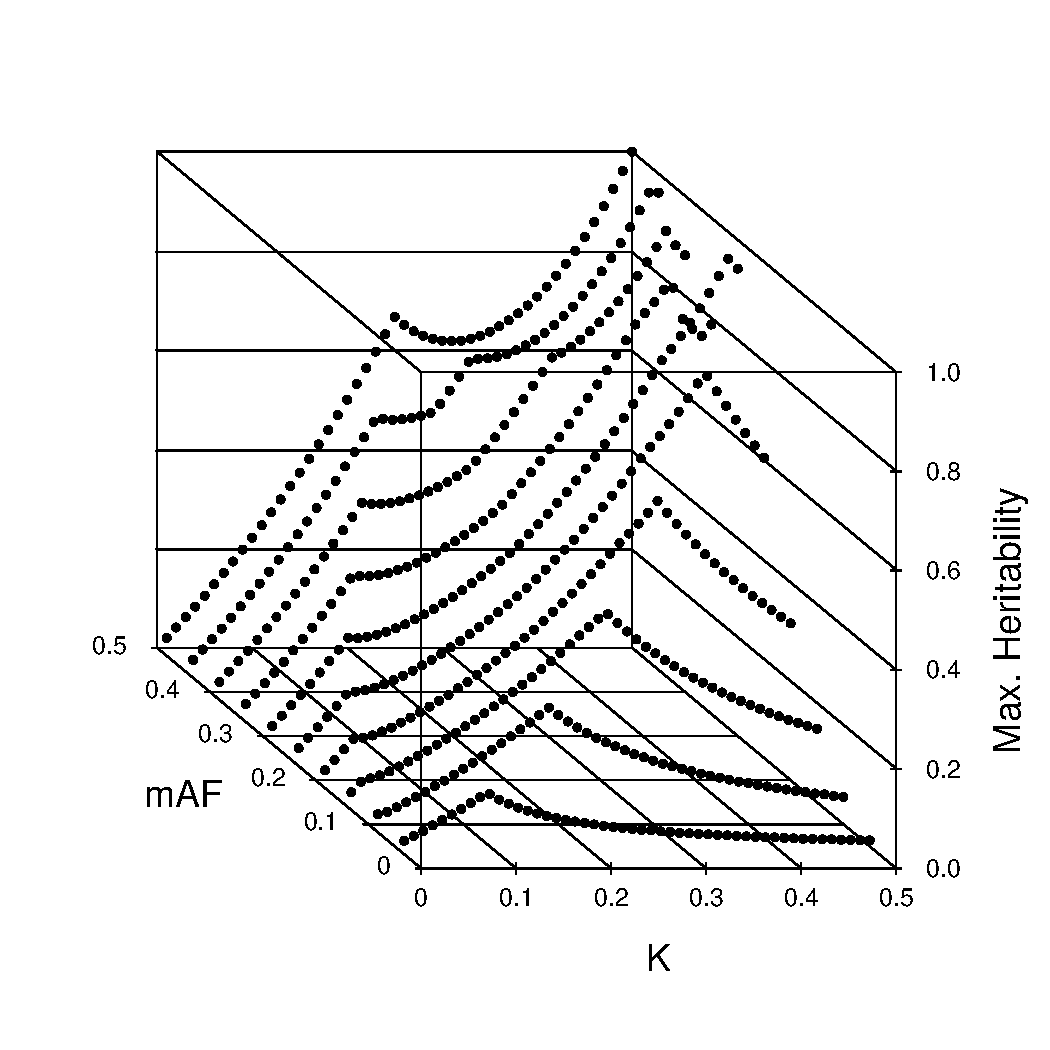
\includegraphics[width=0.7\textwidth]{Figure8_UG.pdf}}% %16.6  FigMaxHerFinal.pdf
\caption{Plot of our maximum heritability estimates for pure, strict, 2-locus models.}
\label{maxherfig}
\end{figure}

\section{Command-Line Operation}\label{cmdop}
GAMETES may also be run from the command line.  If your goal is to generate an archive of genetic models and simulated datasets, than it would be advantageous to code a wrapper script calling GAMETES from the command line.  To obtain a list of commands for command line operation, type \texttt{java -jar GAMETES$\_$2.1.jar -h}.  Like the GUI, running GAMETES from the command line affords users the ability to independently generate genetic models and then separately generate simulated datasets.  Note that custom models may not be generated from the command line.  However, custom model files may be generated with the GUI and then used to generate datasets from the command line.

Below is the help printout for GAMETES specifying the various command line arguments.\\ \\
\begin{scriptsize}
\begin{verbatim}


Usage: java -jar gametes.jar [-h, --help]
[{-M, --model} " [{-h, --heritability} float] [{-p, --prevalence} float]
[{-a, --attributeAlleleFrequency} float] [{-d, --useOddsRatio}] [{-o, --outputFile} filename] [{-f, --proportion} float]] "

[{-q, --rasQuantileCount} integer] [{-p, --rasPopulationCount} integer] [{-t, --rasTryCount} integer]
[{-r, --randomSeed} integer]
[{-i, --modelInputFile} filename] [{-f, --modelInputFileFraction} float] [{-v, --predictiveInputFile} filename] 
[{-z, --noiseInputFile} filename] [{-u, --testingOutputFile} filename]

[{-D, --dataset} [{-n, --alleleFrequencyMin} float] [{-x, --alleleFrequencyMax} float]
[{-a, --totalAttributeCount} integer] [{-m, --missingValueRate}] [{-t, --totalCount}] [{-s, --caseCount} integer]
[{-w, --controlCount} integer] [{-r, --replicateCount} integer]
[{-c, --continuous}] [{-h, --mixedModelDatasetType} [heterogenous, hierarchical]] 
[{-d --standardDeviation} double] [{-[, --rangeMinimum} double] 
[{-], --rangeMaximum} double] [{-o, --datasetOutputFile} filename]"]




\end{verbatim}
\end{scriptsize}

\subsection{Generate a Single Model File}
When running GAMETES from the command line, the user has a number of options.  First we will explain the simplest scenario, where GAMETES is applied to generate models given certain model constraints.  Consider the following example...

\begin{center}
\texttt{java -jar GAMETES$\_$2.1.jar -M " -h 0.2 -p 0.3 -a 0.3 -a 0.2 -o myModel" -q 2 -p 1000 -t 100000}
\end{center}

This command directs GAMETES to generate a 2-locus model with heritability (-h) of 0.2, population prevalence (-p) of 0.3, one SNP with MAF (-a) of 0.3, and the second with MAF (-a) of 0.2.  The number of loci in the model is specified by the number of MAF values specified (e.g. if three -a constraints were added, GAMETES would search for 3-locus models).  Note, that the model constraints are given following -M, with all model constraints given within quotes. Next, comes commands dealing with how models are generated, selected, and saved.  In this example, GAMETES would output 2 model architectures (-q), selected as quantiles from the model population which are saved to an output file (-o) named "mySimulatedModel.txt" in the working directory.  These models would be selected from a population (-p) of 1000 models generated by GAMETES with the above model constraints.  Since GAMETES does not generate a successful model every attempt, in this example we have limited GAMETES to 100,000 model generation attempts (-t), at which point it will stop trying to reach its goal of 1000 models, and select the 2 specified model architectures, assuming it has found at least 2 in its search. By default, model generation from the command line uses the EDM difficulty metric to rank models.  In order to use the COR metric simply add -d to the above command as follows:

\begin{center}
\texttt{java -jar GAMETES$\_$2.1.jar -M " -h 0.2 -p 0.3 -a 0.3 -a 0.2 -d -o otherModel.txt" -q 2 -p 1000 -t 100000}
\end{center}

\subsection{Generate Datasets From a Single Model File}
Now, lets assume we want to generate simulated datasets from a single, previously saved model file.  Consider the following example which generates datasets including randomly generated non-predictive attributes, from the models we generated in the first command line example above.

\begin{center}
\texttt{java -jar GAMETES$\_$2.1.jar -i myModel\_Models.txt -D " -n 0.01 -x 0.5 -a 100 -s 500 -w 500 -r 100 -o myData"}
\end{center}

This command would direct GAMETES to generate 100 replicate datasets (-r) from each model architecture found within the input model file (-i) named "mySimulatedModel.txt".   In this example all dataset constraints are given following -D with all constraints given within quotes.  For each of the datasets generated, non-predictive SNPs will have a minimum MAF (-n) of 0.01, and a maximum MAF (-x) of 0.5.  Each will also have a total of 100 attributes (-a), predictive and non-predictive combined, along with 500 cases (-s) and 500 controls (-w).  (-o) gives the output file name for the dataset files.

\subsection{Do Both: Generate a Model File and Associated Datasets}
Instead of doing both tasks separately, you can generate a model as well as associated datasets in one command as follows...

\begin{center}
\texttt{java -jar GAMETES$\_$2.1.jar -M " -h 0.2 -p 0.3 -a 0.3 -a 0.2 -o myModel.txt" -q 2 -p 1000 -t 100000  -D " -n 0.01 -x 0.5 -a 100 -s 500 -w 500 -r 100 -o myData"}
\end{center}

\subsection{Generate Non-Predictive Attributes From A Loaded Dataset}
Again here we are generating data from a single model file.  However instead of randomly generating non-predictive attributes, lets assume that you wish to load an existing file (such as a real SNP dataset) to be used as the non-predictive attributes.

\begin{center}
\texttt{java -jar GAMETES$\_$2.1.jar -i myModel\_Models.txt -z myRealData.txt -D " -p 0.5 -o myData"}
\end{center}

This example loads myRealData.txt which must be formatted as described in section \ref{loaddata} and adds predictive attributes simulated from the model in myModel\_Models.txt.  If there are multiple quantile models in myModel\_Models.txt, a single simulated dataset will be generated for each.  In this example -p is no longer the prevalence of a model, rather the prevalence of  sick/case samples.  This give the user the option to adjust the case/control ratio within the simulated dataset.  When loading a data for non-predictive attributes, the number of instances in the data is limited by the number of instances in the loaded dataset file.  If the user sets -p to 0.5, GAMETES will generate a balanced dataset (i.e. 50\% cases and 50\% controls) assuming myRealData.txt contained an even number of samples.  Also note that -n, -x, -a, -s, -w, and -r are no longer applicable since the non-predictive attributes are completely determined by the loaded file.

\subsection{Generate Heterogeneous Datasets from Existing Model Files}
Assuming that the user wants to generate heterogeneous datasets combining previously generated model files, this can be performed as in the following example...

\begin{center}
\texttt{java -jar GAMETES$\_$2.1.jar -i myModel\_Models.txt -f 75 -i otherModel\_Models.txt -f 25 -D "-n .05 -x 0.5 -a 100 -s 200 -w 200 -r 100 -o myHetData"}
\end{center}

\subsection{Do Both: Generate Multiple Models and Associated Heterogeneous Datasets}
Again, both tasks can be combined as a single command.  The following example will generate two model files and use them to generate heterogeneous datasets.

\begin{center}
\texttt{java -jar GAMETES$\_$2.1.jar -M " -h 0.1 -p 0.5 -a 0.3 -a 0.1 -f 75 -o myModel.txt" -M " -h 0.03 -p 0.5 -a 0.5 -a 0.5 -a 0.5 -f 25 -o otherModel.txt" -q 2 -p 1000 -t 100000 -D "-n 0.01 -x 0.5 -a 100 -s 500 -w 500 -r 100 -o myHetData"}
\end{center}

\subsection{Generate Models and Associated Datasets with Continous-Valued Endpoints}
The following example will generate a model file and use it to generate a dataset with continuous-valued endpoints.
The command -c indicates that the user wants to generate datasets with continuous-valued endpoints rather than binary discrete datasets. Note that -h can either be defined as heterogeneous or hierarchical if there are multiple models. \\
Within the Dataset commands, -d indicates the standard deviation around model penetrance values used to simulate continuous-valued endpoints. Larger standard deviation values will yield noisier datasets.

\begin{center}
\texttt{java -jar GAMETES$\_$2.1.jar -M " -h 0.05 -p 0.3 -a 0.3  -o myModel.txt" -q 1 -p 100000 -t 100000000 -D " -n 0.01 -x 0.5 -a 100 -c -d 0.5 -t 2000 -r 30 -o contEndpointData"}
\end{center}

\subsection{Generate Hierarchical Datasets}

This example takes in two model files, myModel\_Models.txt and otherModel\_Models.txt, as input and uses them to generate hierarchical datasets. The command -h is defined as hierarchical in this case, and can also be defined as heterogeneous if there are multiple models. 

\begin{center}
\texttt{java -jar GAMETES$\_$2.1.jar -i myModel\_Models.txt -f 75 -i otherModel\_Models.txt -f 25 -D " -h hierarchical -n 0.01 -x 0.5 -a 100 -s 500 -w 50 -w 50 -r 50 -o additiveData"}
\end{center}


\chapter{Future GAMETES Expansions} 
The following sections describe expansions of the GAMETES software intended to be made available in future versions.

\section{Impure and Nested Epistasis} 
While pure, strict epistasis makes a logical gold standard for complex multi-locus interaction models, users may want to generate models that don't meet these strict specifications.  The GAMETES algorithm may be easily expanded to generate impure, nested epistatic models as well.  \emph{Impure} epistasis implies that one or more of the interacting loci have a main effect contributing to disease status.  \emph{Nested} refers to epistasis in which at least one proper subset of the loci also interact epistatically.

\bibliographystyle{plain}  % Style BST file
\bibliography{GAMETES_ref}

%\begin{thebibliography}{}
%\end{thebibliography}
\end{document}